\documentclass[12pt,a4paper]{article}
\title{%
  Arduinoøving 1 \\
  \large IELET1002 - Datateknikk \\
  }
\author{Gunnar Myhre, BIELEKTRO}

\usepackage{graphicx}
\usepackage[utf8]{inputenc}
\usepackage[norsk]{babel}
\usepackage{amsmath}
\usepackage[siunitx]{circuitikz}
\graphicspath{ {./arduino_img} }

\setlength\parindent{0pt}

%https://github.com/trihedral/ArduinoLatexListing/blob/master/arduinoLanguage.tex
% Patch for æøå: \lstset{texcl=true}
\input{arduinoLanguage.tex}

\begin{document}
  \maketitle
  \section{Oppgåve 1}
  \textbf{a)}
  Pull-down--knapp
  \begin{itemize}
    \item brytar åpen $\rightarrow$ LED på
    \item brytar lukka $\rightarrow$ LED av
  \end{itemize}


  \begin{lstlisting}[language=Arduino, basicstyle=\tiny]
const int buttonPin = 2;
const int ledPin = 13;
const int delayTimeMs = 10;

bool buttonState = 0;

void setup() {
  pinMode(ledPin, OUTPUT);
  pinMode(buttonPin, INPUT);
}

void loop() {
  buttonState = digitalRead(buttonPin);
  if (buttonState == 0) {
    digitalWrite(ledPin, LOW);
  } else {
    digitalWrite(ledPin, HIGH);
  }
  delay(delayTimeMs);
}
  \end{lstlisting}
  \begin{center}
    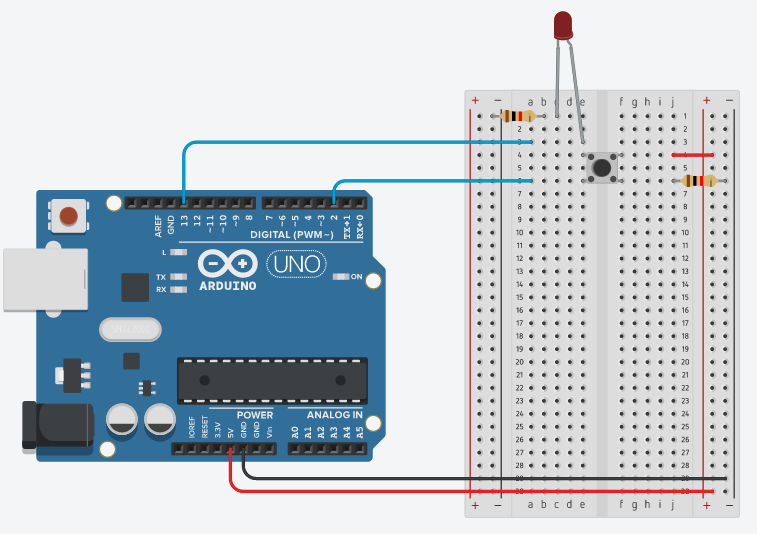
\includegraphics[width=200pt]{01_1_a.png}
  \end{center}

  \newpage
  \textbf{b)}
  Pull-up--knapp
  \begin{itemize}
    \item brytar åpen $\rightarrow$ LED av
    \item brytar lukka $\rightarrow$ LED på
  \end{itemize}


  \begin{lstlisting}[language=Arduino, basicstyle=\tiny]
const int buttonPin = 2;
const int ledPin = 13;
const int delayTimeMs = 10;

bool buttonState = 0;

void setup() {
  pinMode(ledPin, OUTPUT);
  pinMode(buttonPin, INPUT);
}

void loop() {
  buttonState = digitalRead(buttonPin);
  if (buttonState == 1) {
    digitalWrite(ledPin, LOW);
  } else {
    digitalWrite(ledPin, HIGH);
  }
  delay(delayTimeMs);
}
  \end{lstlisting}
  \begin{center}
    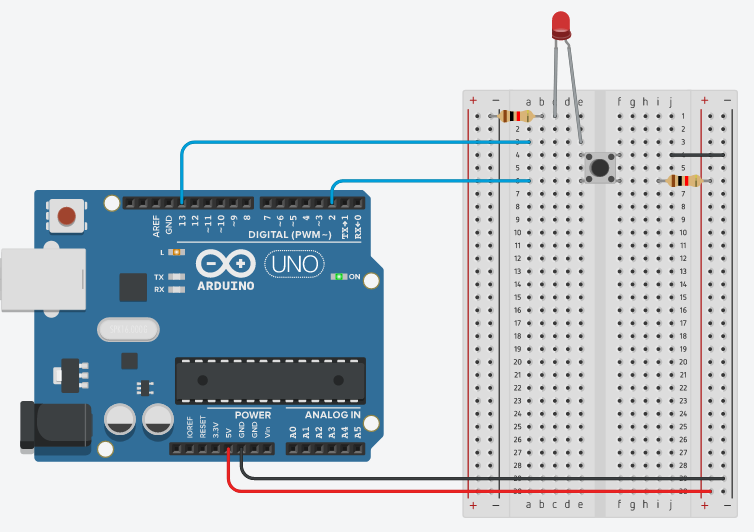
\includegraphics[width=200pt]{01_1_b.png}
  \end{center}

  \newpage
  \textbf{c)}
  Pull-down--knapp med blinkande LED
  \begin{itemize}
    \item brytar åpen $\rightarrow$ LED på
    \item brytar lukka $\rightarrow$ LED blinker
  \end{itemize}

  \begin{lstlisting}[language=Arduino, basicstyle=\tiny]
const int buttonPin = 2;
const int ledPin = 13;
const int delayTimeMs = 10;

bool buttonState = 0;
bool ledState = 0;

void setup() {
  pinMode(ledPin, OUTPUT);
  pinMode(buttonPin, INPUT);
}

void loop() {
  buttonState = digitalRead(buttonPin);
  if (buttonState == 0) {
    // Blink LED
    digitalWrite(ledPin, ledState);

    // Toggle ledState
    ledState = !ledState;

    delay(100);
  } else {
    digitalWrite(ledPin, HIGH);
  }
  delay(delayTimeMs);
}
  \end{lstlisting}
    
  \textbf{d)}
  Pull-down--knapp med blinkande LED
  \begin{itemize}
    \item brytar åpen $\rightarrow$ LED på
    \item brytar lukka $\rightarrow$ LED blinker
    \item brytar åpen igjen $\rightarrow$ LED av
  \end{itemize}

  \begin{lstlisting}[language=Arduino, basicstyle=\tiny]
const int buttonPin = 2;
const int ledPin = 13;
const int delayTimeMs = 10;

bool buttonState = 0;
bool buttonInhibit = 0;
bool ledState = 0;

void setup() {
  pinMode(ledPin, OUTPUT);
  pinMode(buttonPin, INPUT);
}

void loop() {
  buttonState = digitalRead(buttonPin);
  if (buttonState == 1) {
    buttonInhibit = 1;
    // Blink LED
    digitalWrite(ledPin, ledState);

    // Toggle ledState
    ledState = !ledState;

    delay(100);
  } else {
    if (buttonInhibit) {
  	digitalWrite(ledPin, LOW);
    } else {
  	digitalWrite(ledPin, HIGH);
    }
  }
  delay(delayTimeMs);
}
  \end{lstlisting}

  \newpage

  \textbf{e)}
  Pull-down--knapp med blinkande LED
  \begin{itemize}
    \item brytar 1 åpen $\rightarrow$ LED på
    \item brytar 1 lukka $\rightarrow$ LED blinker
    \item brytar 1 åpen igjen $\rightarrow$ LED av
    \item brytar 2 lukka $\rightarrow$ LED på igjen
  \end{itemize}

  \begin{lstlisting}[language=Arduino, basicstyle=\tiny]
const int blinkButtonPin = 2;
const int resetButtonPin = 3;
const int ledPin = 13;
const int delayTimeMs = 10;

bool blinkButtonState = 0;
bool resetButtonState = 0;
bool ledInhibit = 0;
bool ledState = 0;

void setup() {
  pinMode(ledPin, OUTPUT);
  pinMode(blinkButtonPin, INPUT);
  pinMode(resetButtonPin, INPUT);
}

void loop() {
  blinkButtonState = digitalRead(blinkButtonPin);
  resetButtonState = digitalRead(resetButtonPin);

  if (blinkButtonState == 1) {
    ledInhibit = 1;
    // Blink LED
    digitalWrite(ledPin, ledState);

    // Toggle ledState
    ledState = !ledState;

    delay(100);
  } else {
    if (ledInhibit) {
      //Inhibit the LED
  	  digitalWrite(ledPin, LOW);
    } else {
  	digitalWrite(ledPin, HIGH);
    }
  }
  if (resetButtonState == 1) {
    //Remove the inhibitor so the LED can be activated again
    ledInhibit = 0;
  }
  delay(delayTimeMs);
}
  \end{lstlisting}

  \begin{center}
    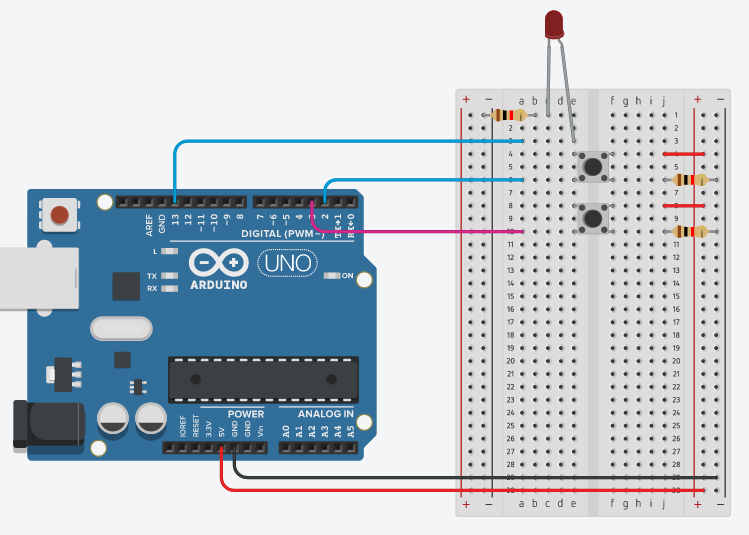
\includegraphics[width=200pt]{01_1_e.png}
  \end{center}

  \section{Oppgåve 2}
  \textbf{a)}
  Fotoresistor med indikator-LED for to terskelverdiar
  \begin{itemize}
    \item $lysverdi < terskel_1 \rightarrow$ LED av
    \item $terskel_1 < lysverdi < terskel_2 \rightarrow$ LED på
    \item $lysverdi > terskel_2 \rightarrow$ LED blinker
  \end{itemize}

  \begin{lstlisting}[language=Arduino, basicstyle=\tiny]
const int photoresistorPin = A0;
const int ledPin = 13;
const int blinkDelayMs = 200;

float treshold_1 = 1000;
float treshold_2 = 1500;
float lightSensorReading = 0;
int ledState = 0;

void setup() {
  pinMode(ledPin, OUTPUT);
  pinMode(photoresistorPin, INPUT);
}

void loop() {
  lightSensorReading = analogRead(photoresistorPin);

  if (lightSensorReading >= treshold_1) {
    if (lightSensorReading >= treshold_2) {
      
      //If sensor value is above treshold 2, blink the LED
      ledState = !ledState;
      digitalWrite(ledPin, ledState);
      
    } else {
      //If sensor value is between treshold 1 and 2, LED on
      digitalWrite(ledPin, HIGH);      
    }
  } else {
    //If sensor value is under treshold 1, LED off
    digitalWrite(ledPin, LOW);    
  }
  delay(blinkDelayMs);
}
  \end{lstlisting}
  \begin{center}
    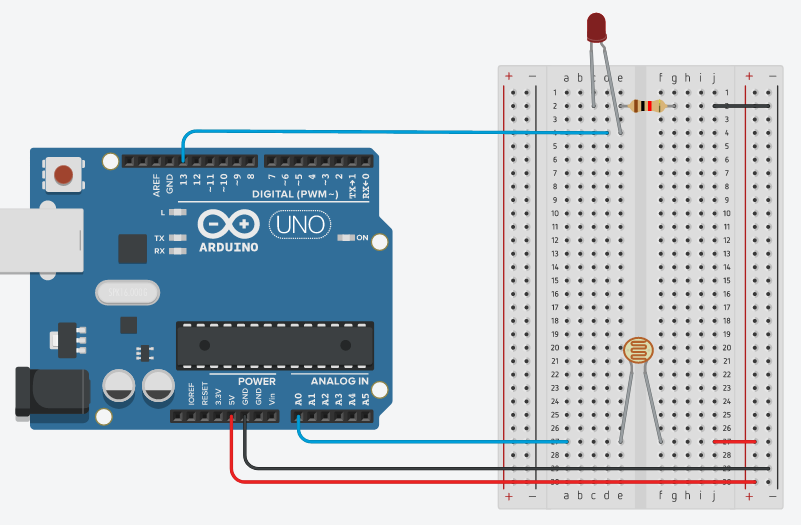
\includegraphics[width=200pt]{01_2_a.png}
  \end{center}

  \newpage

  \textbf{b)}
  Potensiometerkrets
  \begin{lstlisting}[language=Arduino, basicstyle=\tiny]
// Deklarerer variablar
const int potMeterPin = A0;
int potMeterReading;

void setup() {
  //Deklarerer modus for potmeter-pinnen
  pinMode(potMeterPin, INPUT);

  //Initialiserer seriellmonitoren over 9600 baud
  Serial.begin(9600);
}

void loop() {
  //Gjer ei måling på potmeter-pinnen
  potMeterReading = analogRead(potMeterPin);

  //Printer målingsverdien over seriellmonitoren
  Serial.println(potMeterReading);

  //Venter eitt millisekund
  delay(1);
}
  \end{lstlisting}
  \begin{center}
    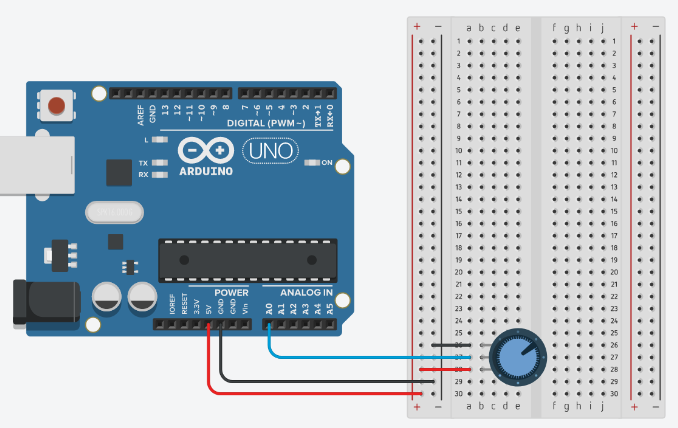
\includegraphics[width=200pt]{01_2_b.png}
  \end{center}
  Når programmet køyrer vert verdiar avlest frå $A0$ kontinuerleg printa til
  seriellmonitoren. Eg observerer at verdiane går ifrå 0 på jordsida til
  1023 på kildesida. Dette er eit verdispenn på 1024, altså $2^{10}$. Dette
  kan skyldast måten Arduino UNO sin ADC (analog-til-digital--konverterar)
  er implementert.

  \begin{center}
    \begin{circuitikz} \draw
      (0,0) to[potentiometer, n=pot, l=10<\kilo\ohm>] ++ (4,0)
            to[short, -*] (4,-0.2)
      (pot.wiper) to[short, -o] ++ (2,0)

      (0,0) node[ground]{}
      (4,-1) node[label=$V_{ss}$]{}
      (4.5,0.3) node[label=$A0$]{}

      (6,0) to[R, l=5<\kilo\ohm>] (8,0)
            to[R, l=5<\kilo\ohm>] (10,0)
            to[short, -*] (10,-0.2)
      (8,0) -- (8,1) to[short, -o] ++ (2,0)

      (6,0) node[ground]{}
      (10,-1) node[label=$V_{ss}$]{}
      (10.5,0.6) node[label=$A0$]{}
      ;
    \end{circuitikz}
  \end{center}

  Kretsteikningane over viser eit potmeter og ein spenningsdelar. Desse to kretsane
  er ekvivalente dersom eit $10\si{\kilo\ohm}$--potensiometer står i 50$\%$--posisjon.
  Eg gjennomfører testen frå oppgåveteksten.

  \begin{itemize}
    \item Kopler av kilden, nå står $R_{pot}$ mellom GND og A0. Det skal ikkje
      gå nokon straum igjennom $R_{pot}$ og spenninga skal då vere $0V = GND$. Dette
      ser vi også i seriellmonitoren som printer 0.
    \item Kopler av GND. Nå står $R_{pot}$ mellom A0 og 5V. Det skal ikkje gå nokon
      straum inn i ADC-en, og derfor vil spenningsfallet vere 0. Spenninga som står
      i A0 skal derfor vere 5V. Verdien som skrivast til seriellmonitoren er 1023.
  \end{itemize}

  Sidan den simulerte arduinoen i Tinkercad opererer ideelt (den er m.a. i stand til å
  forsyne kretsen med $125 \si{\kilo\watt}$) vil ikkje verdiane i testen avvike frå
  verdiane når potmeteret er kopla mellom GND og 5V. På ein faktisk arduino kan verdiane
  avvike pga arduinoens straumforsyning som må forsyne tilstrekkelig effekt.

  \begin{equation}
    P=\frac{v^2}{R}=\frac{(5V)^2}{10\si{\kilo\ohm}} = 2,5\si{\milli\watt}
  \end{equation}

  \textbf{c)}

  For å måle faktiske spenningsverdiar mellom 0V og 5V må vi ta hensyn til at målingas
  verdispenn er 1024.

  \begin{equation}
    1023k=5 \Rightarrow k=\frac{5}{1023}=0,004887586
  \end{equation}

  I arduino vert dette

  \begin{lstlisting}[language=Arduino, basicstyle=\small]
//Rekner ut spenning i A0 og printer til Serial
pinVoltage = potMeterReading * 0.004887586;
Serial.println(pinVoltage);
  \end{lstlisting}
  Det vi måler her er spenningsfallet over den delen av $R_{pot}$ som til ein kvar
  tid befinner seg mellom A0 og 5V. \\


  \textbf{d)}

  For å finne motstandsverdiane kan vi bruke formel for spenningsdeling

  \begin{equation}
    v_{A0} = \frac{R_1}{R_{pot}}v_s \rightarrow R_1 = \frac{v_f R_{pot}}{v_s}
  \end{equation}
  Dette er motstanden mellom A0 og GND. Vi subtraherer frå $R_{pot}$ for å finne
  verdien mellom A0 og 5V. I arduino kan vi skrive det slik:

  \begin{lstlisting}[language=Arduino, basicstyle=\small]
//Rekner ut motstand mellom A0 og Vss og printer til Serial
potMeterResistance = 10000 - (pinVoltage * 10000) / 5;
Serial.println(potMeterResistance);
  \end{lstlisting}

  \newpage

  Heile koden for \textbf{c)} og \textbf{d)} ser slik ut:
  \begin{lstlisting}[language=Arduino, basicstyle=\small]
// Deklarerer variablar
const int potMeterPin = A0;
int potMeterReading;
float pinVoltage;
float potMeterResistance;

void setup() {
  //Deklarerer modus for potmeter-pinnen
  pinMode(potMeterPin, INPUT);

  //Initialiserer seriellmonitoren over 9600 baud
  Serial.begin(9600);
}

void loop() {
  //Gjer ei måling på potmeter-pinnen
  potMeterReading = analogRead(potMeterPin);

  //Rekner ut spenning i A0
  pinVoltage = potMeterReading * 0.004887586;

  //Rekner ut motstanden mellom A0 og Vss
  potMeterResistance = 10000 - (pinVoltage * 10000) / 5;
  
  //Printer målingsverdiane over seriemonitoren
  Serial.print("voltage: ");
  Serial.print(pinVoltage);
  Serial.print(" resistance: ");
  Serial.println(potMeterResistance);

  //Venter eitt millisekund
  delay(1);
}


  \end{lstlisting}

  \newpage

  \section{Oppgåve 3}
  \textbf{a)} Blinkekrets med stadig aukande frekvens, $1 - x^2$. Krav: ingen
  while-løkke (skjønt arduinos loop er ei while-løkke).

  \begin{lstlisting}[language=Arduino, basicstyle=\small]
//Constants
const int ledPin = 13;

//Variables
int ledState = 0;
int blinkInterval;
int blinkIterator;
float maxDelay = 1000;
int minDelay = 50;
int stepSize = 1;

void setup() {
  pinMode(ledPin, OUTPUT);
}

void loop() {
  //If delay interval passes minDelay, reset it and the iterator
  if (blinkInterval < minDelay) {
    blinkInterval = maxDelay;
    blinkIterator = 0;
  }
  
  //Quadratic function: 1 - x**2
  blinkInterval = maxDelay - pow(blinkIterator, 2);

  //Blink the LED
  digitalWrite(ledPin, HIGH);
  delay(blinkInterval);
  digitalWrite(ledPin, LOW);
  delay(blinkInterval);
  
  //Increment the iterator
  blinkIterator += stepSize;
}
  \end{lstlisting}

  \newpage

  \textbf{b)} Blinkekrets med stadig lengre oppholdsintervall, $x^2$.
  Her er det enkelt å bytte om på grensene og starte grafen frå
  null i staden for 1 s. Eg bytter óg plass på dei to blokkene slik
  at eit potensielt kjempehøgt oppholdsintervall vert luka ut i
  if-setninga.

  \begin{lstlisting}[language=Arduino, basicstyle=\small]
  //Quadratic function: x**2
  blinkInterval = pow(blinkIterator, 2);

  //If delay surpasses maxDelay, reset it and the iterator
  if (blinkInterval > maxDelay) {
    blinkInterval = minDelay;
    blinkIterator = 0;
  }
  \end{lstlisting}

  \begin{center}
    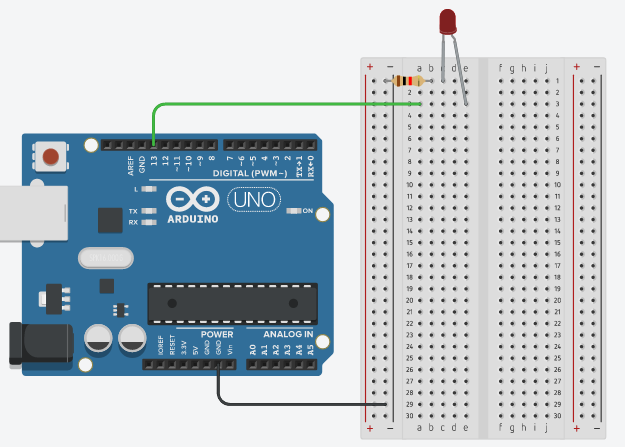
\includegraphics[width=200pt]{01_3_a.png}
  \end{center}
  Oppkopling av arduino for oppg. 3.


\end{document}
